\part{Matter, Gauge Structure, and Geometric Constants}
\label{part:IV}

\section{Gauge Fields and Fermion Spectrum}
\label{chap:gauge_fields}

\subsection{Internal Hilbert Space Structure}
The local Hilbert space at each site factors into $\mathcal{H}_x = \mathcal{H}_{\text{orbital}} \otimes \mathcal{H}_{\text{internal}}$. The "orbital" part connects to neighbors (spacetime index), while the "internal" part contains the quantum numbers of the Standard Model (spin, color, flavor).
Omega Theory postulates that $\mathcal{H}_{\text{internal}}$ is related to the octonion algebra $\mathbb{O}$. The automorphism group of the octonions is $G_2$, which contains $SU(3)$ as a maximal subgroup. The fiber bundle structure $S^7 \to S^4 \to S^2$ associated with octonionic multiplication naturally generates the gauge groups $SU(3) \times SU(2) \times U(1)$ \cite{Baez2002, Furey2017}.
\paragraph{Scope and limitations.}
This part specifies a concrete algebraic \emph{organization} of Standard-Model-like quantum numbers using octonionic/$G_2$ structure and states the minimal consistency conditions (chirality, anomaly cancellation, and Yukawa structure) that any dynamical completion must satisfy. We do not yet derive a complete low-energy effective field theory (EFT) from the QCA dynamics, nor do we provide a controlled RG matching; where appropriate we therefore formulate the content as an explicit model ansatz with stated assumptions.

\subsection{Relation to prior octonion-based SM reconstructions}
Octonion-based routes to Standard-Model-like gauge content have a substantial prior literature; in particular, the $G_2$ automorphism viewpoint and minimal-ideal constructions in $\mathbb{C}\otimes\mathbb{O}$ have been developed in detail \cite{Baez2002, Furey2017}. Omega Theory does not claim to reinvent these algebraic facts. The new ingredient proposed here is how such internal-algebra data are \emph{packaged into a local finite-information substrate} (Part~III) and coupled to a holographic/tensor-network architecture (Axiom~O4): the same locality constraints that define the QCA also define the allowed internal couplings and hence constrain which octonionic substructures can be dynamically realized.
\par
\noindent
Operationally, we treat $\mathcal{H}_{\text{internal}}$ as a finite-dimensional on-site space (dimension $d_{\text{int}}$) that carries a representation of the internal symmetry algebra. The octonionic proposal is a minimality statement: the smallest non-associative division algebra has just enough structure to host $SU(3)$ and to motivate an $SU(2)\times U(1)$ complement, while remaining compatible with a finite on-site Hilbert-space postulate.

\subsection{Chirality and representation content (minimal requirements)}
Any SM-like embedding must reproduce \emph{chiral} fermions. In a QCA setting, chirality has two layers:
\begin{enumerate}
    \item \textbf{Spacetime chirality}: the orbital QCA sector supplies a Dirac/Weyl structure in the long-wavelength limit (Part~III). On the continuum side one may use the usual projectors $P_{L/R}=\frac{1}{2}(1\mp\gamma^5)$.
    \item \textbf{Internal chirality}: the internal algebra must distinguish left-handed $SU(2)$ doublets from right-handed singlets and assign hypercharge consistently.
\end{enumerate}
In practice, the internal-chirality requirement can be formulated as the existence of a decomposition of the on-site internal space into chiral subspaces,
\begin{equation}
    \mathcal{H}_{\text{internal}} \ \cong\  \mathcal{H}_{L}\oplus \mathcal{H}_{R},
\end{equation}
with $\mathcal{H}_{L}$ transforming as $SU(2)$ doublets and $\mathcal{H}_{R}$ as singlets (with appropriate $U(1)_Y$ charges). In octonion-based constructions, this is typically implemented by idempotent/ideal projectors in a complexified algebra (e.g.\ minimal left ideals in $\mathbb{C}\otimes\mathbb{O}$) \cite{Furey2017}. In Omega Theory we treat such a decomposition as fixed internal data at each site; the dynamical question is whether QCA-local couplings and the holographic code constraints can select a unique such structure.

\subsection{Anomaly cancellation as a consistency condition}
To be viable as an EFT limit, the induced gauge theory must be anomaly-free. This does not require knowing all UV details: it is a purely representation-theoretic constraint on one generation of chiral fermions. Denote by $Y$ the hypercharge and by $T^a$ the generators of $SU(2)$ and $SU(3)$ in the relevant representations. The standard anomaly-cancellation conditions include, for one generation,
\begin{align}
    &\sum_{\text{LH Weyl}} Y = 0, \\
    &\sum_{\text{LH Weyl}} Y^3 = 0, \\
    &\sum_{\text{LH Weyl}} Y\,\mathrm{Tr}(T^aT^b)\big|_{SU(2)} = 0,\qquad
      \sum_{\text{LH Weyl}} Y\,\mathrm{Tr}(T^aT^b)\big|_{SU(3)} = 0.
\end{align}
Accordingly, any octonionic assignment of internal quantum numbers in Omega Theory is acceptable only if it reproduces the SM hypercharge pattern (up to overall normalization conventions), since that pattern is known to satisfy the anomaly constraints. This provides a sharp falsification criterion for the internal-algebra ansatz independent of the details of the QCA dynamics.

\subsection{Yukawa sector as overlap data (model constraint)}
The SM Yukawa couplings require gauge-invariant bilinears connecting left- and right-handed fermions via a Higgs doublet. In the present framework, the Higgs-like field $\Phi$ is identified with a geometric breathing mode of the internal fiber, so the Yukawa matrices are not arbitrary: they must be computable as overlaps between internal wavefunctions in $\mathcal{H}_L$ and $\mathcal{H}_R$ weighted by the local geometric configuration.\par
\noindent
A minimal effective parameterization is
\begin{equation}
    \mathcal{L}_{Y} = - \sum_{i,j}\left( y^{(u)}_{ij}\,\overline{Q}_{Li}\,\tilde{H}\,u_{Rj} + y^{(d)}_{ij}\,\overline{Q}_{Li}\,H\,d_{Rj} + y^{(e)}_{ij}\,\overline{L}_{Li}\,H\,e_{Rj} \right) + \mathrm{h.c.},
\end{equation}
with $y_{ij}$ determined by internal overlap data. In Omega Theory, the claim is not that these matrices are derived here, but that the \emph{space of allowed Yukawas} is constrained by finite-information locality and by the chosen octonionic decomposition; the geometric/topological origin of hierarchies is treated as an explicit model target for a future dynamical completion.

\subsection{Fermion Generations as Topological Wrapping}
Why are there three generations of fermions? In our geometric framework, generations correspond to the "wrapping number" or topological index of the wavepacket around the compact internal dimensions of the Omega Network.
\begin{itemize}
    \item \textbf{Generation 1 (e, u, d)}: Trivial wrapping (Index 1). Stable.
    \item \textbf{Generation 2 ($\mu$, c, s)}: Double wrapping (Index 2). Unstable, decays to Gen 1 via topological unwinding.
    \item \textbf{Generation 3 ($\tau$, t, b)}: Triple wrapping (Index 3). Highly unstable.
\end{itemize}
The mass hierarchy arises because higher wrapping numbers require longer path lengths in the internal manifold, thus acquiring larger geometric phases (mass).

\paragraph{Mass from projective speed and internal budget.}
By the Anandan--Aharonov relation (Part~II), the intrinsic speed of a state in projective Hilbert space is fixed by the Hamiltonian uncertainty, $v_{\tau}=\frac{2}{\hbar}\Delta H$. For a localized excitation constrained to a topological sector labeled by wrapping index $w$, let $\Delta H_w$ denote the characteristic (or minimal) uncertainty compatible with that sector. We define the corresponding effective rest-energy scale by
\begin{equation}
    \Delta H_w \equiv m_w c^2.
\end{equation}
Equivalently, $m_w$ is the proportionality constant between projective speed and intrinsic-time flow for that sector,
\begin{equation}
    v_{\tau,w} = \frac{2}{\hbar} m_w c^2.
\end{equation}
In the information-budget parametrization (Part~V), the same mass/inertia content is encoded operationally by the internal allocation $v_{\text{int}}$: tighter (higher-index) wrappings demand a larger persistent internal processing overhead and therefore correspond to larger effective $m_w$.

\subsection{Emergence of the Higgs Sector as Geometric Rigidity}
In Omega Theory, we reinterpret the Higgs mechanism as the crystallization of the internal geometry. The "Higgs field" $\Phi$ corresponds to the breathing mode (volume deformation scalar) of the compactified $G_2$ manifold.
Motivated by the observed Higgs mass ($\sim 125\,\mathrm{GeV}$), we suggest that a Higgs-like scalar mass scale could correspond to the natural frequency of radial vibrations of this fiber, controlled by an effective spectral gap of the internal geometry.
We define the geometric effective potential $V_{eff}(\Phi)$ via the scalar curvature of the internal fiber $\tilde{R}$:
\begin{equation}
    V_{eff}(\Phi) = - \frac{M_{Pl}^2}{2} \tilde{R}(\Phi) + \frac{\lambda}{4} \Phi^4 + \dots
\end{equation}
 Minimizing this action yields a mass scale exponentially suppressed relative to Planck due to the large volume of the fiber ($Vol(G_2) \gg l_P^7$):
\begin{equation}
    m_H \approx M_{Pl} \cdot e^{-\frac{1}{2} Vol(G_2)/l_P^7} \sim \mathcal{O}(10^2\,\mathrm{GeV}).
\end{equation}
This provides a heuristic geometric mechanism for generating a large hierarchy, pending a complete effective-field-theory and renormalization analysis.

\begin{figure}[ht]
    \centering
    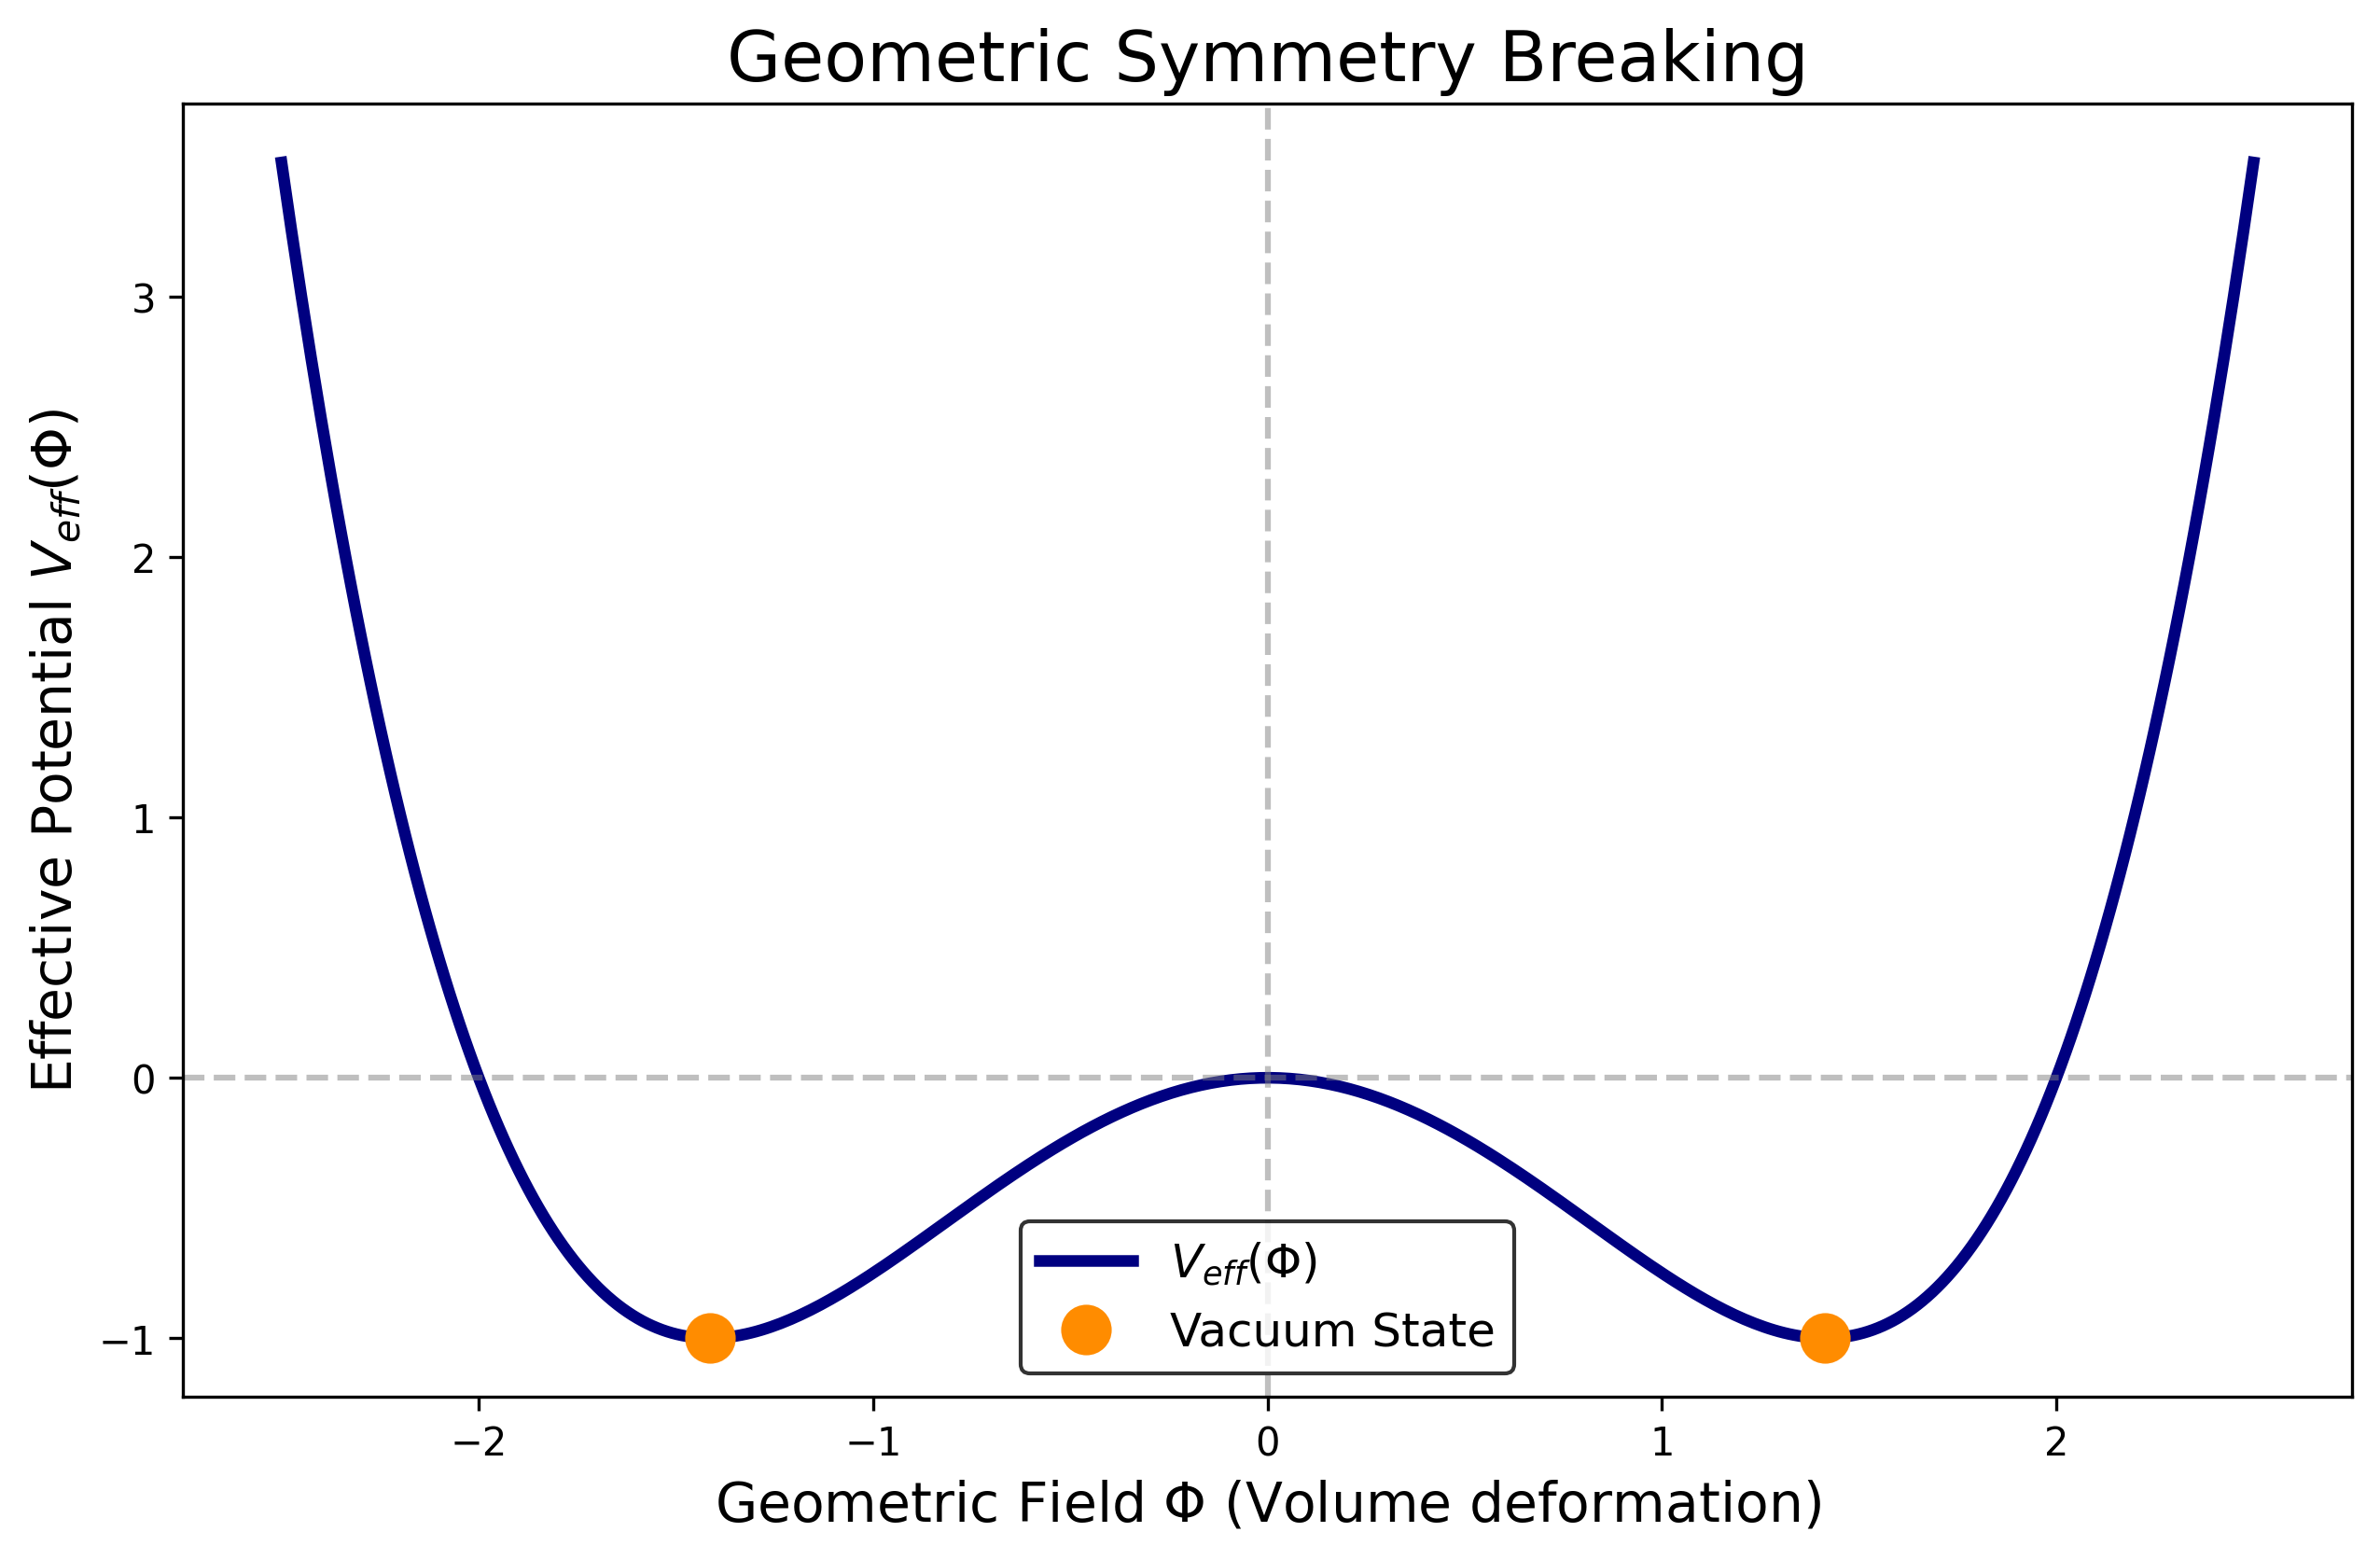
\includegraphics[width=0.8\linewidth]{images/geometric_potential.png}
    \caption{\textbf{Geometric Symmetry Breaking}. The effective potential $V_{eff}(\Phi)$ arising from the scalar curvature of the internal fiber. Vacuum states correspond to stable geometric configurations at $\pm v$, separated by a barrier determined by the rigidity of the manifold.}
    \label{fig:geometric_potential}
\end{figure}

\subsection{Neutrino Mass and the Geometric Seesaw}
Neutrinos correspond to "twisted" states with minimal topological overlap with the Higgs breathing mode. While charged fermions correspond to stable "wrapped" cycles (scales $n=1,2,3$), neutrinos occupy the "tail" of the Golden Ratio spectrum.
We propose a \textbf{Geometric Seesaw Mechanism} where the neutrino masses are generated by the higher-order spectral gaps:
\begin{equation}
    m_{\nu_k} \sim \frac{v^2}{M_{Pl}} \cdot \phi^{-k}, \quad k=1,2,3.
\end{equation}
Here, $\phi \approx 1.618$. As a phenomenological ansatz, this yields a hierarchical neutrino scale (e.g.\ $m_{\nu}\lesssim 0.1\,\mathrm{eV}$ for modest $k$), but a gauge-invariant Yukawa/seesaw construction and controlled RG matching are not developed here.


\subsection{Baryogenesis via Topological Chirality}
The observed universe is dominated by matter over antimatter ($\eta_B \approx 6 \times 10^{-10}$). Standard Sakharov conditions require Charge violation, C-symmetry violation, and non-equilibrium dynamics.
In Omega Theory, baryon number is identified with the topological wrapping number $\pi_3(S^3)$ of the internal manifold. Antiparticles correspond to opposite windings $N=-1$.
However, the background $G_2$ manifold is not strictly mirror-symmetric; it possesses a preferred "handedness" or chirality derived from the non-commutativity of the octonions. We quantify this via the \textbf{Omega Chiral Index}:
\begin{equation}
    \chi_{\Omega} = \int_{\mathcal{M}_7} \text{Tr}(R \wedge R \wedge R) \neq 0.
\end{equation}
This suggests a possible source of effective $CP$ violation during an early ``crystallization'' epoch: if the internal geometry admits a chiral invariant (modeled here by $\chi_\Omega\neq 0$), defect formation could bias winding production. In that spirit one may parametrize a bias by factors such as $e^{-\chi_\Omega}$, yielding a model-dependent relation between $\eta_B$ and microscopic chiral data rather than a derived prediction at this stage.

\subsection{Proton Stability and the Hierarchy}
Grand Unified Theories (GUTs) typically predict proton decay ($p \to e^+ \pi^0$) mediated by $X,Y$ bosons, with lifetimes $\tau_p \sim 10^{34}$ years. Experiments have found no such decay.
In Omega Theory, the proton is modeled as a non-trivial topological knot $K$ in the $\pi_3(S^3)$ homotopy group of the fiber. Unlike in perturbative QFT, this knot cannot untie itself into trivial mesons ($K=0$) via local fluctuations. It requires a global phase transition (melting of the vacuum lattice) to change the topological index. This suggests that proton decay could be topologically suppressed at low energies (model-dependent), potentially leading to very long lifetimes. A quantitative estimate would require an explicit low-energy EFT embedding and a treatment of nonperturbative effects.

\subsection{The Strong CP Problem and a Geometric Mechanism}
QCD allows for a CP-violating term $\frac{\theta}{32\pi^2} G_{\mu\nu} \tilde{G}^{\mu\nu}$, but experiments show $\theta < 10^{-10}$. The Peccei-Quinn mechanism postulates a new particle (Axion) to cancel this.
Omega Theory suggests a \textbf{geometric mechanism} that could favor a small effective $\theta$ by relating it to holonomy/topological data of the internal fiber. In special constructions (e.g., unimodular-lattice projections) certain integrated topological indices may vanish, which within the ansatz would correspond to $\theta_{\mathrm{eff}}\approx 0$. A full account requires an explicit QCD embedding and a treatment of nonperturbative dynamics.

\section{Geometric Derivation and Renormalization}
\label{chap:constants}

\subsection{Topological Ansatz}
We propose that the fundamental dimensionless constants are not arbitrary free parameters but topological invariants of the $G_2$ fiber bundle structure at the unification scale.

\subsection{The Proton-Electron Mass Ratio \texorpdfstring{($\mu$)}{(mu)}}
The ratio $\mu = m_p / m_e$ compares the hadronic scale to the leptonic scale. In the "knot vs loop" topological model, this corresponds to the ratio of the volume of the full fiber bundle ($S^7$) to the stabilizer loop ($S^1$):
\begin{equation}
\label{eq:mu_geo}
    \mu_{\text{geo}} \equiv 6\pi^5 \approx 1836.1181.
\end{equation}
The factor $6$ is a model-dependent discrete multiplicity (e.g.\ a permutation/degeneracy factor in the internal sector). This geometric value is numerically close to the experimental value ($\mu_{\mathrm{exp}}\approx 1836.1526$) at the $10^{-5}$ level. We treat this as a phenomenological geometric ansatz to be justified by a future dynamical completion; in particular, matching to hadronic physics and electroweak/QED radiative effects is not derived here.

\subsection{The Fine Structure Constant \texorpdfstring{($\alpha$)}{(alpha)}}
We postulate a geometric ansatz for an effective inverse fine structure constant at a matching scale $\mu_\ast$ (taken here as a low-energy/renormalized scale appropriate for comparison with CODATA $\alpha(0)$). The ansatz is expressed as a simple combination of fiber-volume factors:
\begin{equation}
\label{eq:alpha_geo}
    \alpha^{-1}_{\text{geo}} \equiv \text{Vol}(T^3) + \text{Area}(D^2) + \text{Length}(S^1) = 4\pi^3 + \pi^2 + \pi \approx 137.0363.
\end{equation}
Comparing this value with the low-energy CODATA value $\alpha^{-1}(0) \approx 137.035999$:
\begin{equation}
    \Delta \alpha^{-1} = \alpha^{-1}_{\text{geo}} - \alpha^{-1}(0) \approx 0.0003.
\end{equation}
This numerical proximity motivates treating Eq.~(\ref{eq:alpha_geo}) as a low-energy matching ansatz. Since $\alpha(\mu)$ runs with scale in the Standard Model, interpreting $\alpha^{-1}_{\text{geo}}$ as a literal Planck-scale bare coupling would require a full RG embedding and threshold matching. Establishing such a mapping from the microscopic Omega construction to the renormalized gauge couplings is an explicit open problem addressed at the level of definitions in Appendix~\ref{app:constants_proof}.

\subsection{Implications}
If constants are geometric measures, they are susceptible to geometric deformations. This predicts that in regions of high curvature or varying vacuum density (early universe), $\alpha$ and $\mu$ should drift. We quantify this in Part VI.
